% ReRoom architecture figures -- TikZ / LaTeX reproduction of the SVG diagrams,
% so they render natively in a PDF submission (no Unicode/font breakage).
% Compile:  pdflatex arch_figures.tex   (needs tikz; standalone class)
% Or \input the individual tikzpicture blocks into your paper.
\documentclass[border=4pt]{standalone}
\usepackage{tikz}
\usepackage{amsmath,amssymb}
\usetikzlibrary{arrows.meta,positioning,fit,backgrounds,calc}

\definecolor{teal}{HTML}{2A6F7A}
\definecolor{rust}{HTML}{A8412A}
\definecolor{grn}{HTML}{2A7A2A}
\definecolor{panel}{HTML}{FBFBFA}

% ---- shared styles ----
\tikzset{
  box/.style   ={draw=black,line width=.6pt,rounded corners=2pt,align=center,
                 font=\footnotesize,inner sep=3pt},
  net/.style   ={draw=teal,line width=1pt,rounded corners=4pt},
  rel/.style   ={draw=teal,line width=.8pt,fill=teal!7,rounded corners=2pt,
                 align=center,font=\footnotesize,inner sep=3pt},
  dit/.style   ={draw=rust,line width=.8pt,fill=rust!6,rounded corners=2pt,
                 align=center,font=\footnotesize,inner sep=3pt},
  proj/.style  ={draw=grn,line width=1pt,dashed,fill=grn!8,rounded corners=2pt,
                 align=center,font=\footnotesize,inner sep=3pt},
  head/.style  ={draw=teal,line width=.7pt,align=center,font=\footnotesize,inner sep=3pt},
  band/.style  ={draw=black!12,fill=black!3,rounded corners=3pt,align=left,
                 font=\scriptsize,inner sep=5pt},
  a/.style     ={-{Stealth[length=4pt]},line width=.7pt,gray!60!black},
  atl/.style    ={-{Stealth[length=4pt]},line width=.7pt,teal},
  ar/.style    ={-{Stealth[length=4pt]},line width=.7pt,rust},
  ag/.style    ={-{Stealth[length=4pt]},line width=.7pt,grn},
}

\begin{document}

%============================================================
% FIGURE 2 -- System overview
%============================================================
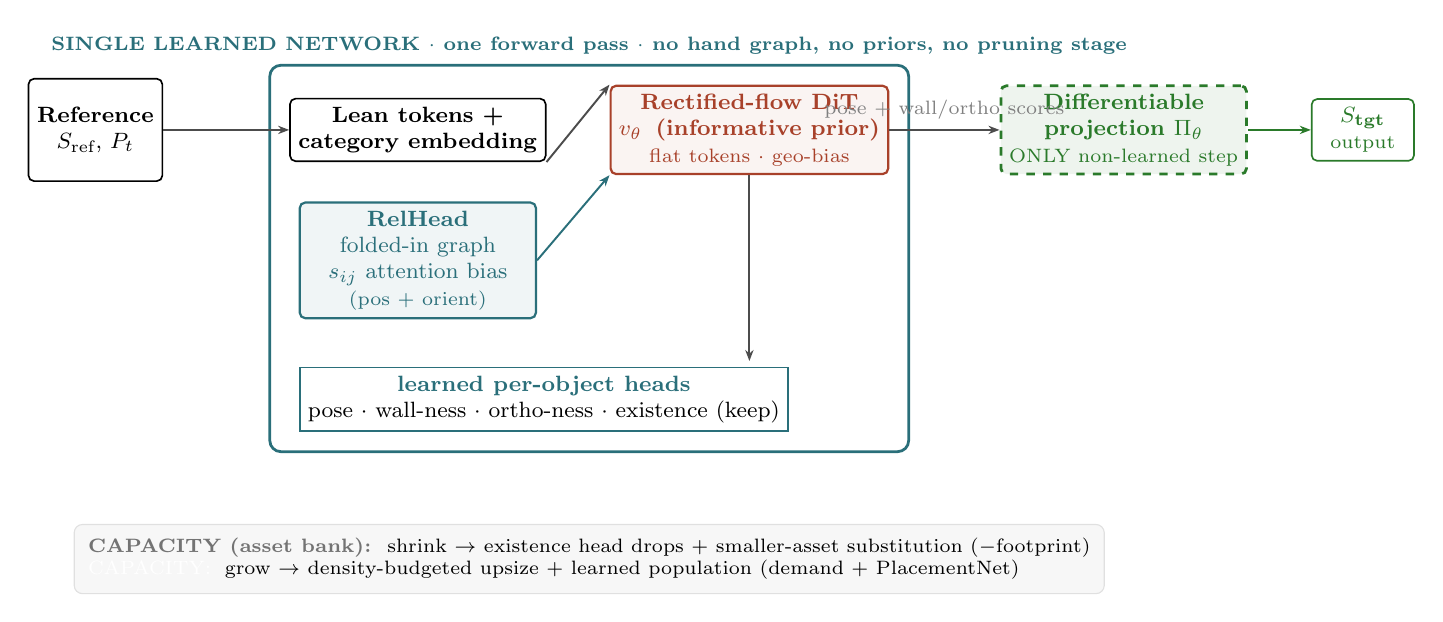
\begin{tikzpicture}[node distance=6mm]
  \node[box,minimum height=13mm,minimum width=17mm] (in)
        {\textbf{Reference}\\ $S_\text{ref},\,P_t$};

  % --- learned network internals ---
  \node[box,right=16mm of in.east,anchor=west,minimum width=30mm] (tok)
        {\textbf{Lean tokens +}\\ \textbf{category embedding}};
  \node[rel,below=5mm of tok,minimum width=30mm] (rel)
        {\textbf{\textcolor{teal}{RelHead}}\\ \textcolor{teal}{folded-in graph}\\
         \textcolor{teal}{$s_{ij}$ attention bias}\\ {\scriptsize\textcolor{teal}{(pos + orient)}}};
  \node[dit,right=8mm of tok.east,anchor=west,minimum width=30mm] (dit)
        {\textbf{\textcolor{rust}{Rectified-flow DiT}}\\
         \textbf{\textcolor{rust}{$v_\theta$\, (informative prior)}}\\
         {\scriptsize\textcolor{rust}{flat tokens $\cdot$ geo-bias}}};
  \node[head,below=6mm of rel.south,anchor=north,minimum width=62mm,xshift=16mm] (heads)
        {\textbf{\textcolor{teal}{learned per-object heads}}\\
         pose $\cdot$ wall-ness $\cdot$ ortho-ness $\cdot$ existence (keep)};

  % container around the learned network
  \begin{scope}[on background layer]
    \node[net,fit=(tok)(rel)(dit)(heads),inner sep=7pt,label={[teal,font=\scriptsize\bfseries]above:SINGLE LEARNED NETWORK $\cdot$ one forward pass $\cdot$ no hand graph, no priors, no pruning stage}] (netbox) {};
  \end{scope}

  % projection + output
  \node[proj,right=14mm of dit.east,anchor=west,minimum width=24mm] (proj)
        {\textbf{\textcolor{grn}{Differentiable}}\\ \textbf{\textcolor{grn}{projection $\Pi_\theta$}}\\
         {\scriptsize\textcolor{grn}{ONLY non-learned step}}};
  \node[box,right=8mm of proj.east,anchor=west,draw=grn,minimum width=13mm]
        (out) {\textbf{\textcolor{grn}{$S_\text{tgt}$}}\\ {\scriptsize\textcolor{grn}{output}}};

  % arrows
  \draw[a] (in.east) -- (tok.west);
  \draw[a] (tok.south east) -- (dit.north west);
  \draw[atl] (rel.east) -- (dit.south west);
  \draw[a] (dit.south) -- ([yshift=2pt]heads.north -| dit.south);
  \draw[a] (dit.east) -- (proj.west)
        node[midway,above,font=\scriptsize,gray]{pose + wall/ortho scores};
  \draw[ag] (proj.east) -- (out.west);

  % capacity band
  \node[band,below=9mm of netbox.south,anchor=north,minimum width=126mm] (cap)
        {\textbf{\textcolor{black!55}{CAPACITY (asset bank):}}\;
         shrink $\to$ existence head drops + smaller-asset substitution ($-$footprint)\\
         \textcolor{white}{CAPACITY:}\; grow $\to$ density-budgeted upsize + learned population (demand + PlacementNet)};
\end{tikzpicture}

%============================================================
% FIGURE 3 -- Relation-conditioned DiT backbone
%============================================================
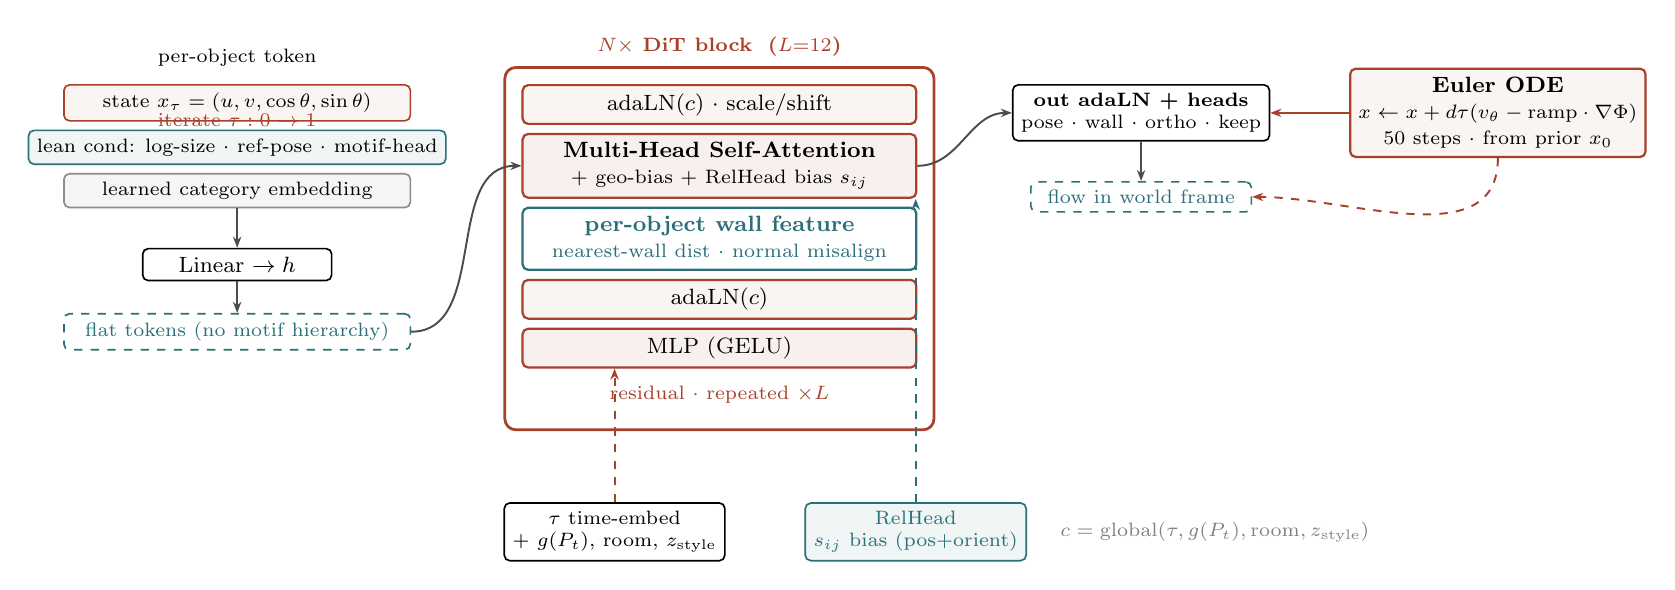
\begin{tikzpicture}[node distance=4mm]
  % token stack
  \node[box,fill=rust!6,draw=rust,minimum width=44mm,font=\scriptsize] (s1)
        {state $x_\tau=(u,v,\cos\theta,\sin\theta)$};
  \node[box,fill=teal!7,draw=teal,below=1mm of s1,minimum width=44mm,font=\scriptsize] (s2)
        {lean cond: log-size $\cdot$ ref-pose $\cdot$ motif-head};
  \node[box,fill=black!4,draw=black!45,below=1mm of s2,minimum width=44mm,font=\scriptsize] (s3)
        {learned category embedding};
  \node[font=\scriptsize,above=1mm of s1] {per-object token};
  \node[box,below=5mm of s3,minimum width=24mm] (lin) {Linear $\to h$};
  \node[box,draw=teal,dashed,below=4mm of lin,minimum width=44mm,font=\scriptsize,text=teal]
        (flat) {flat tokens (no motif hierarchy)};
  \draw[a] (s3.south) -- (lin.north);
  \draw[a] (lin.south) -- (flat.north);

  % DiT block
  \node[dit,right=14mm of s1.north east,anchor=north west,minimum width=50mm] (adal1) {adaLN$(c)$ $\cdot$ scale/shift};
  \node[dit,fill=rust!8,below=1mm of adal1,minimum width=50mm] (attn)
        {\textbf{Multi-Head Self-Attention}\\ {\scriptsize + geo-bias + RelHead bias $s_{ij}$}};
  \node[dit,fill=white,draw=teal,text=teal,below=1mm of attn,minimum width=50mm] (wall)
        {\textbf{per-object wall feature}\\ {\scriptsize nearest-wall dist $\cdot$ normal misalign}};
  \node[dit,below=1mm of wall,minimum width=50mm] (adal2) {adaLN$(c)$};
  \node[dit,fill=rust!8,below=1mm of adal2,minimum width=50mm] (mlp) {MLP (GELU)};
  \node[font=\scriptsize,text=rust,below=1mm of mlp] (res) {residual $\cdot$ repeated $\times L$};
  \begin{scope}[on background layer]
    \node[draw=rust,line width=1pt,rounded corners=4pt,fit=(adal1)(attn)(wall)(adal2)(mlp)(res),inner sep=6pt,
          label={[rust,font=\scriptsize\bfseries]above:$N\times$ DiT block \;($L{=}12$)}] (ditbox) {};
  \end{scope}
  \draw[a] (flat.east) to[out=0,in=180] (attn.west);

  % conditioning
  \node[box,below=9mm of ditbox.south west,anchor=north west,font=\scriptsize] (tau)
        {$\tau$ time-embed\\ {\scriptsize+ $g(P_t)$, room, $z_\text{style}$}};
  \node[box,draw=teal,fill=teal!7,text=teal,right=10mm of tau,font=\scriptsize] (rh)
        {RelHead\\ {\scriptsize $s_{ij}$ bias (pos+orient)}};
  \draw[ar,dashed] (tau.north) -- (mlp.south -| tau.north);
  \draw[atl,dashed] (rh.north) -- (attn.south -| rh.north);
  \node[font=\scriptsize,gray,right=3mm of rh] {$c=\text{global}(\tau,g(P_t),\text{room},z_\text{style})$};

  % output heads + ODE
  \node[box,right=12mm of adal1.north east,anchor=north west,minimum width=28mm,font=\scriptsize] (heads)
        {\textbf{out adaLN + heads}\\ pose $\cdot$ wall $\cdot$ ortho $\cdot$ keep};
  \node[box,draw=teal,dashed,text=teal,below=5mm of heads,minimum width=28mm,font=\scriptsize] (world)
        {flow in world frame};
  \node[dit,right=10mm of heads.east,anchor=west,minimum width=34mm] (ode)
        {\textbf{Euler ODE}\\ {\scriptsize $x\leftarrow x+d\tau(v_\theta-\text{ramp}\cdot\nabla\Phi)$}\\
         {\scriptsize 50 steps $\cdot$ from prior $x_0$}};
  \draw[a] (attn.east) to[out=0,in=180] (heads.west);
  \draw[a] (heads.south) -- (world.north);
  \draw[ar] (ode.west) -- (heads.east);
  \draw[ar,dashed] (ode.south) to[out=270,in=0] (world.east)
        node[pos=.7,below,font=\scriptsize,rust]{iterate $\tau:0\to1$};
\end{tikzpicture}

%============================================================
% FIGURE 4 -- Differentiable proximal projection Pi_theta
%============================================================
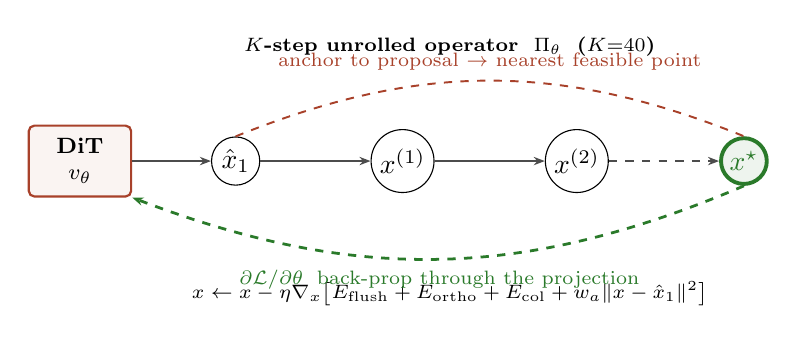
\begin{tikzpicture}
  \node[dit,minimum width=13mm,minimum height=9mm] (dit) {\textbf{DiT}\\ $v_\theta$};
  \node[draw,circle,right=10mm of dit,inner sep=1.5pt] (x0) {$\hat{x}_1$};
  \node[draw,circle,right=14mm of x0,inner sep=1.5pt] (x1) {$x^{(1)}$};
  \node[draw,circle,right=14mm of x1,inner sep=1.5pt] (x2) {$x^{(2)}$};
  \node[draw=grn,line width=1.4pt,circle,fill=grn!8,right=14mm of x2,inner sep=1.5pt,text=grn]
        (xs) {$x^{\star}$};
  \draw[a] (dit.east) -- (x0.west);
  \draw[a] (x0) -- (x1);  \draw[a] (x1) -- (x2);  \draw[a,dashed] (x2) -- (xs);
  \node[font=\scriptsize,text=black,above=8mm of x1,xshift=6mm] {\textbf{$K$-step unrolled operator\; $\Pi_\theta$\; ($K{=}40$)}};
  \node[font=\scriptsize,below=10mm of x1,xshift=6mm]
        {$x\leftarrow x-\eta\nabla_x\!\left[E_\text{flush}+E_\text{ortho}+E_\text{col}+w_a\lVert x-\hat{x}_1\rVert^2\right]$};
  \draw[rust,dashed,line width=.7pt] (x0.north) to[bend left=22]
        node[above,font=\scriptsize,rust,pos=.5]{anchor to proposal $\to$ nearest feasible point} (xs.north);
  \draw[ag,dashed,line width=1pt] (xs.south) to[bend left=22]
        node[below,font=\scriptsize,grn,pos=.5]{$\partial\mathcal{L}/\partial\theta$\; back-prop through the projection} (dit.south east);
\end{tikzpicture}

\end{document}
